\documentclass[10pt]{beamer}

\usetheme{metropolis}
\usepackage{appendixnumberbeamer}

\usepackage{booktabs}
\usepackage[scale=2]{ccicons}
\usepackage{graphicx}
\usepackage{pgfplots}
\usepgfplotslibrary{dateplot}
\usepackage{caption}
\usepackage{subcaption}
\usepackage{xspace}
\usepackage{hyperref,xcolor}

\usepackage{makeidx}
\definecolor{winered}{rgb}{0.5,0,0}
\newcommand{\themename}{\textbf{\textsc{metropolis}}\xspace}

\title{Bhabha Tracking Efficiencies}
%\subtitle{A modern beamer theme}
\date{01.03.2019}
\author{Martin Sobotzik}
\institute{Johannes Gutenberg Universit\"at Mainz}
% \titlegraphic{\hfill
\includegraphics[height=1.5cm]{logo.pdf}}

\definecolor{darkblue}{rgb}{0,0,.5}
\hypersetup{pdftex=true, colorlinks=true, breaklinks=true, linkcolor=darkblue, menucolor=darkblue, pagecolor=darkblue, urlcolor=darkblue}


%citecolor={winered} %Gives errors when turned on
%allcolors={winered} %Gives errors when turned on

\begin{document}

\maketitle
{%
\setbeamertemplate{frame footer}{Bhabha Tracking Efficiencies}

%\section{Reproducing Plots}


\begin{frame}{Motivation}

\begin{itemize}	
	\item I would like to estimate the tracking efficiency Bhabha events
	\item One possible way to do it is to select the electrons using only information coming from the ECL (they are therefore labeled and treated as gammas)
	
	\item Once selected a pure electron sample, one can than look at the Tracks related to ECLClusters
	\item The ratio between the ECLClusters with a Track associated and all the ECLClusters will provide an estimation of tracking efficiency
	\item This idea comes from some plots presented by Sam in previous  \href{https://confluence.desy.de/display/BI/ECL+Meetings?preview=/84320165/109161400/SCunliffe181123-ECL.pdf}{tracking and ECL} meetings. 

\end{itemize}
\end{frame}
	
\begin{frame}{Getting Started}
	
\begin{itemize} 
	\item All cuts were taken from Sam's studies:
	
	
	\begin{itemize}
		\item gamma:probe '$(\textrm{E} > 0.1 )$'
		\item gamma:tag '$(\textrm{clusterE} > 3.0)$'
		\item vpho:cand 'reconstructed from gamma:probe and gamma:tag'
	\end{itemize}

	
		\begin{itemize}
			\item $0.296706 < \theta < 2.61799 \rightarrow$ It has to hit the ECL
			\item $\textrm{nCleanedTracks}[ \textrm{abs}(\textrm{dz}) < 2.0 \textrm{ and } \textrm{abs}(\textrm{dr}) < 0.5 \textrm{ and nCDCHits} > 0 \textrm{ and pt } > 0.15] < 1 \rightarrow $ bad quality hits 
			\item $\textrm{M}(\textrm{vpho}) > 8.0\,\textrm{GeV} \rightarrow $ To cut away background (not from his email but surely he is using something like that)					
		\end{itemize}
	
\end{itemize}	
\end{frame}

\begin{frame}{Reproducing Plots}
	
	\begin{itemize}
		\item The plots in the following slides are produced using prod6 (this is because as a starting point I tried to reproduce Sam's plots)
		\item Sam used all Prod6 data. I am only using the following: /hsm/belle2/bdata/Data/release-02-01-00/DB00000438 /prod00000006/e0003/4S/r02*/all/mdst.sub00/*.root
		\item Sam's plots are on the left.	
		\item Three lines. The middle one is $\textrm{ee} \rightarrow \gamma \gamma$ the two others are $\textrm{ee} \rightarrow \textrm{ee}$
\end{itemize}
	
	
	\begin{figure}
		\centering
		\begin{subfigure}{.5\textwidth}
			\centering
			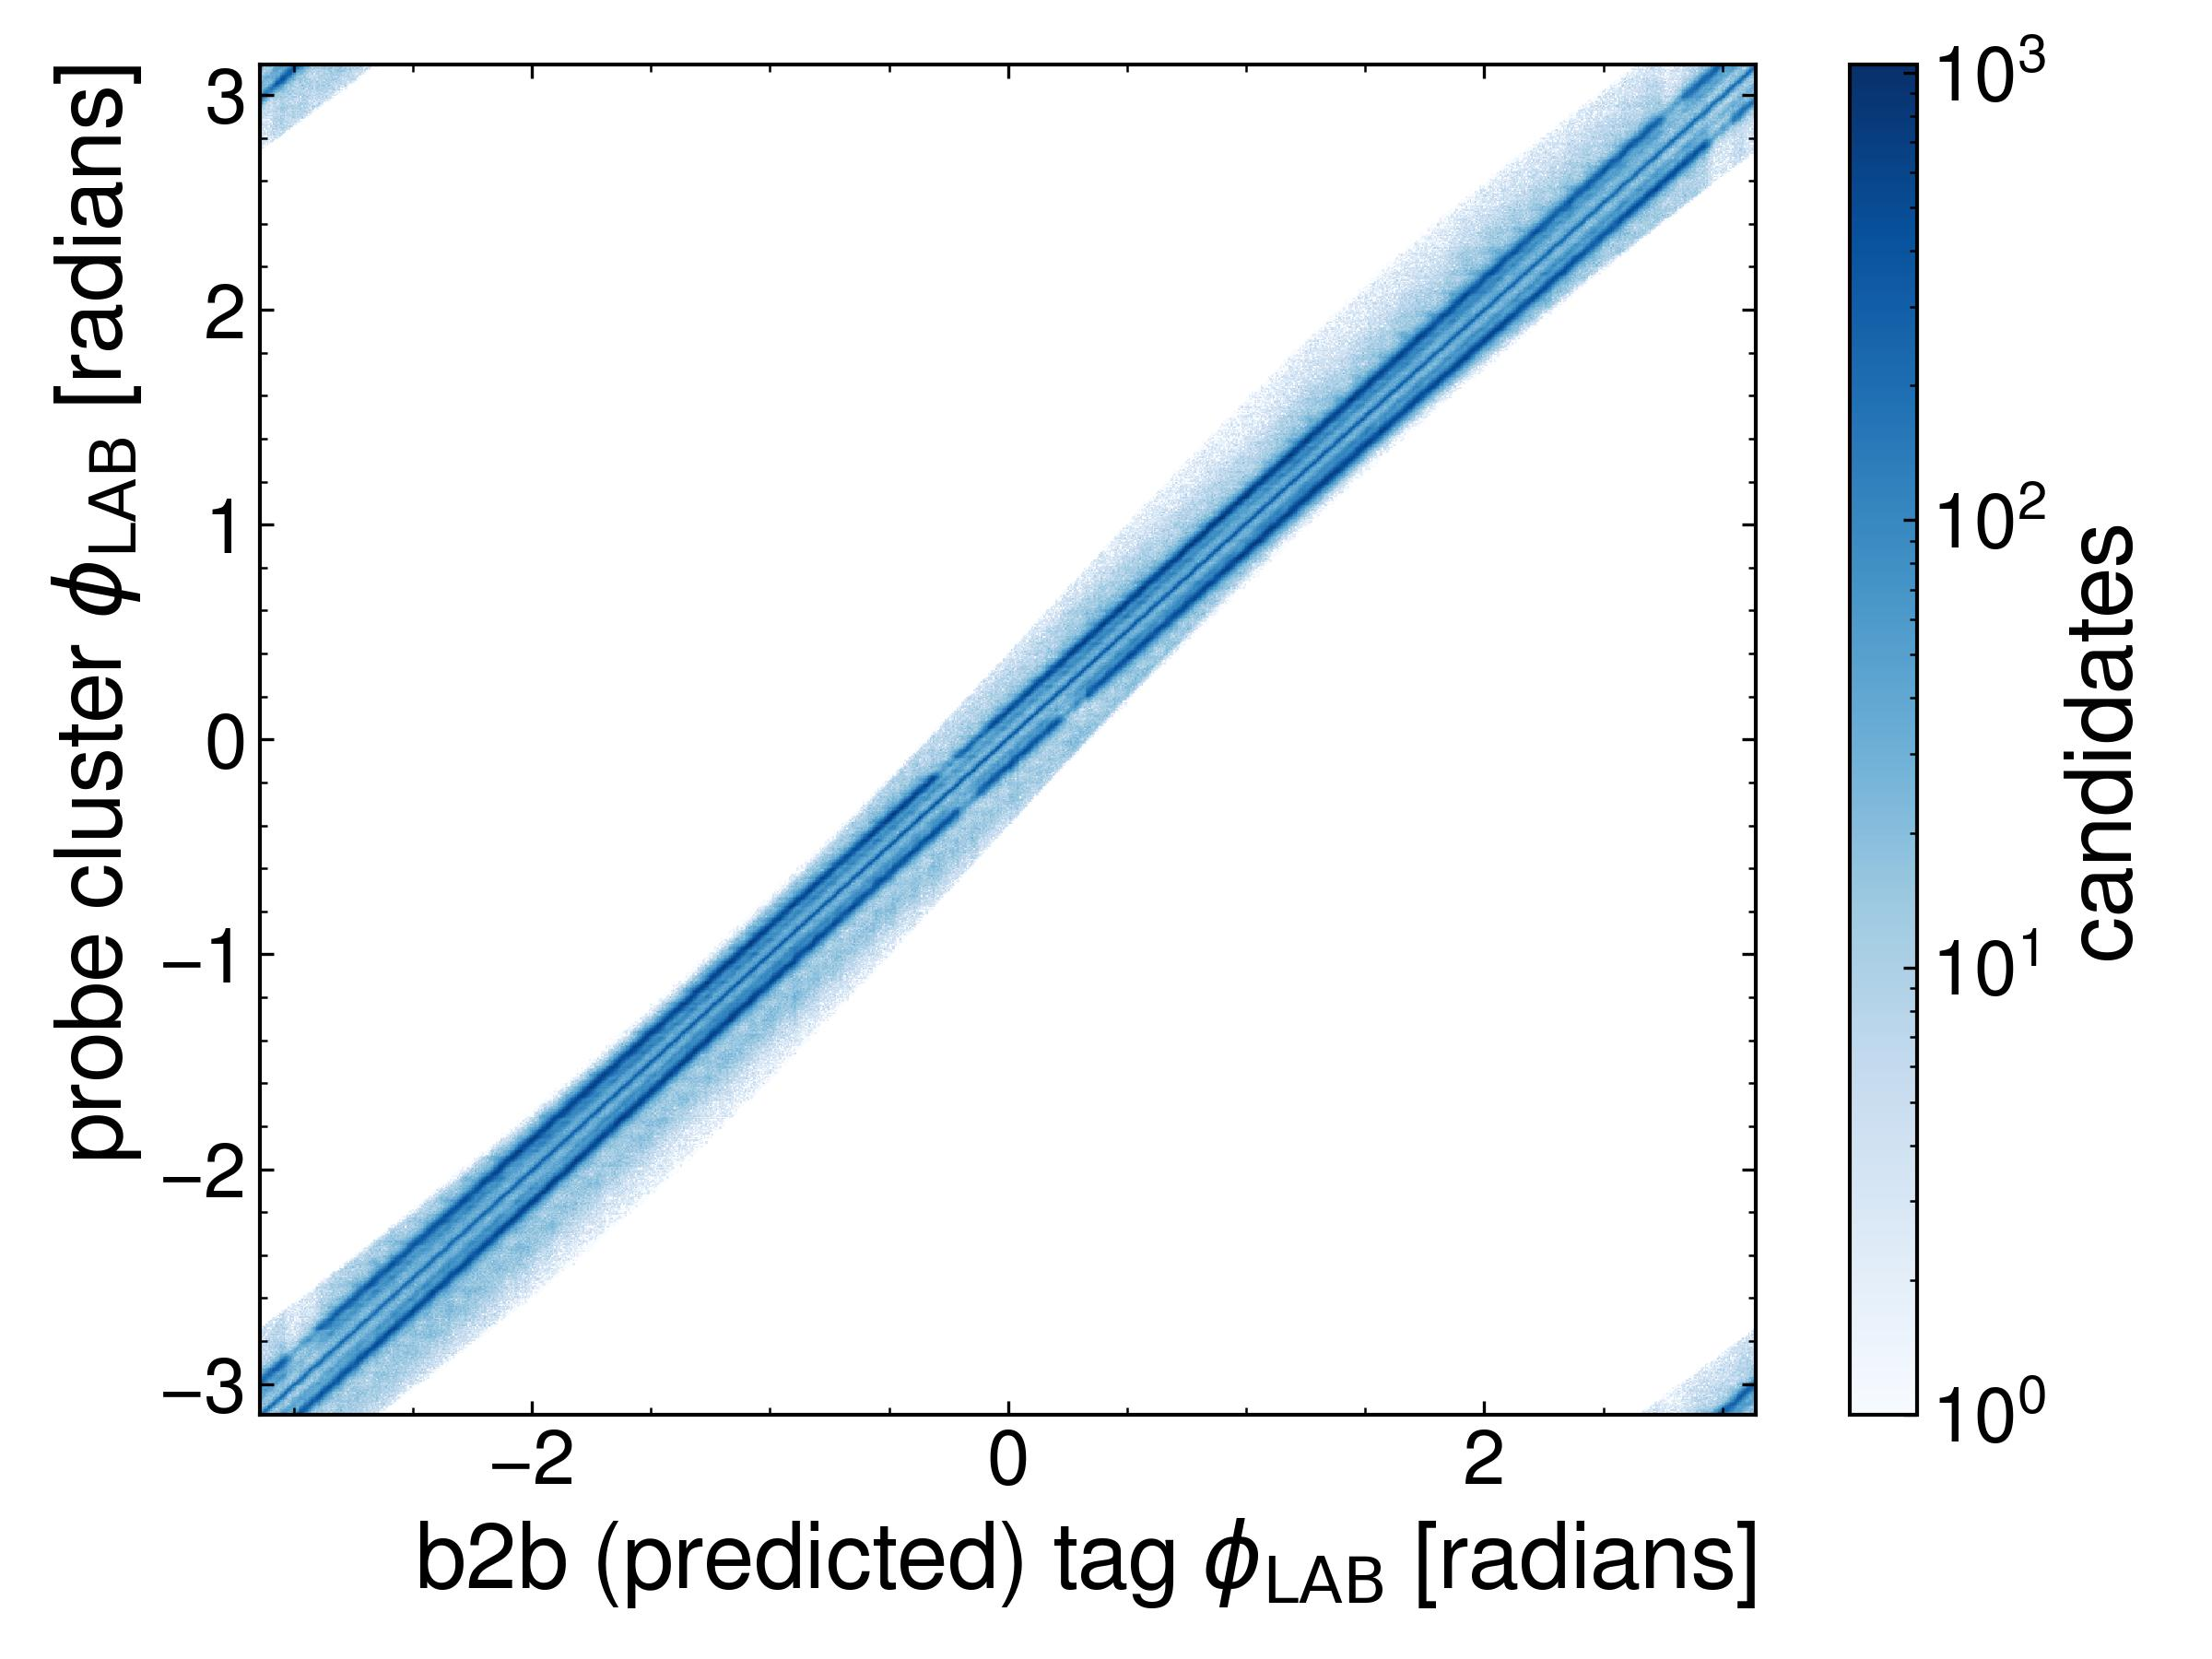
\includegraphics[width=5cm]{Plots/prodRecSam.jpeg}
			
			\label{fig:sub1}
		\end{subfigure}%
		\begin{subfigure}{.5\textwidth}
			\centering
			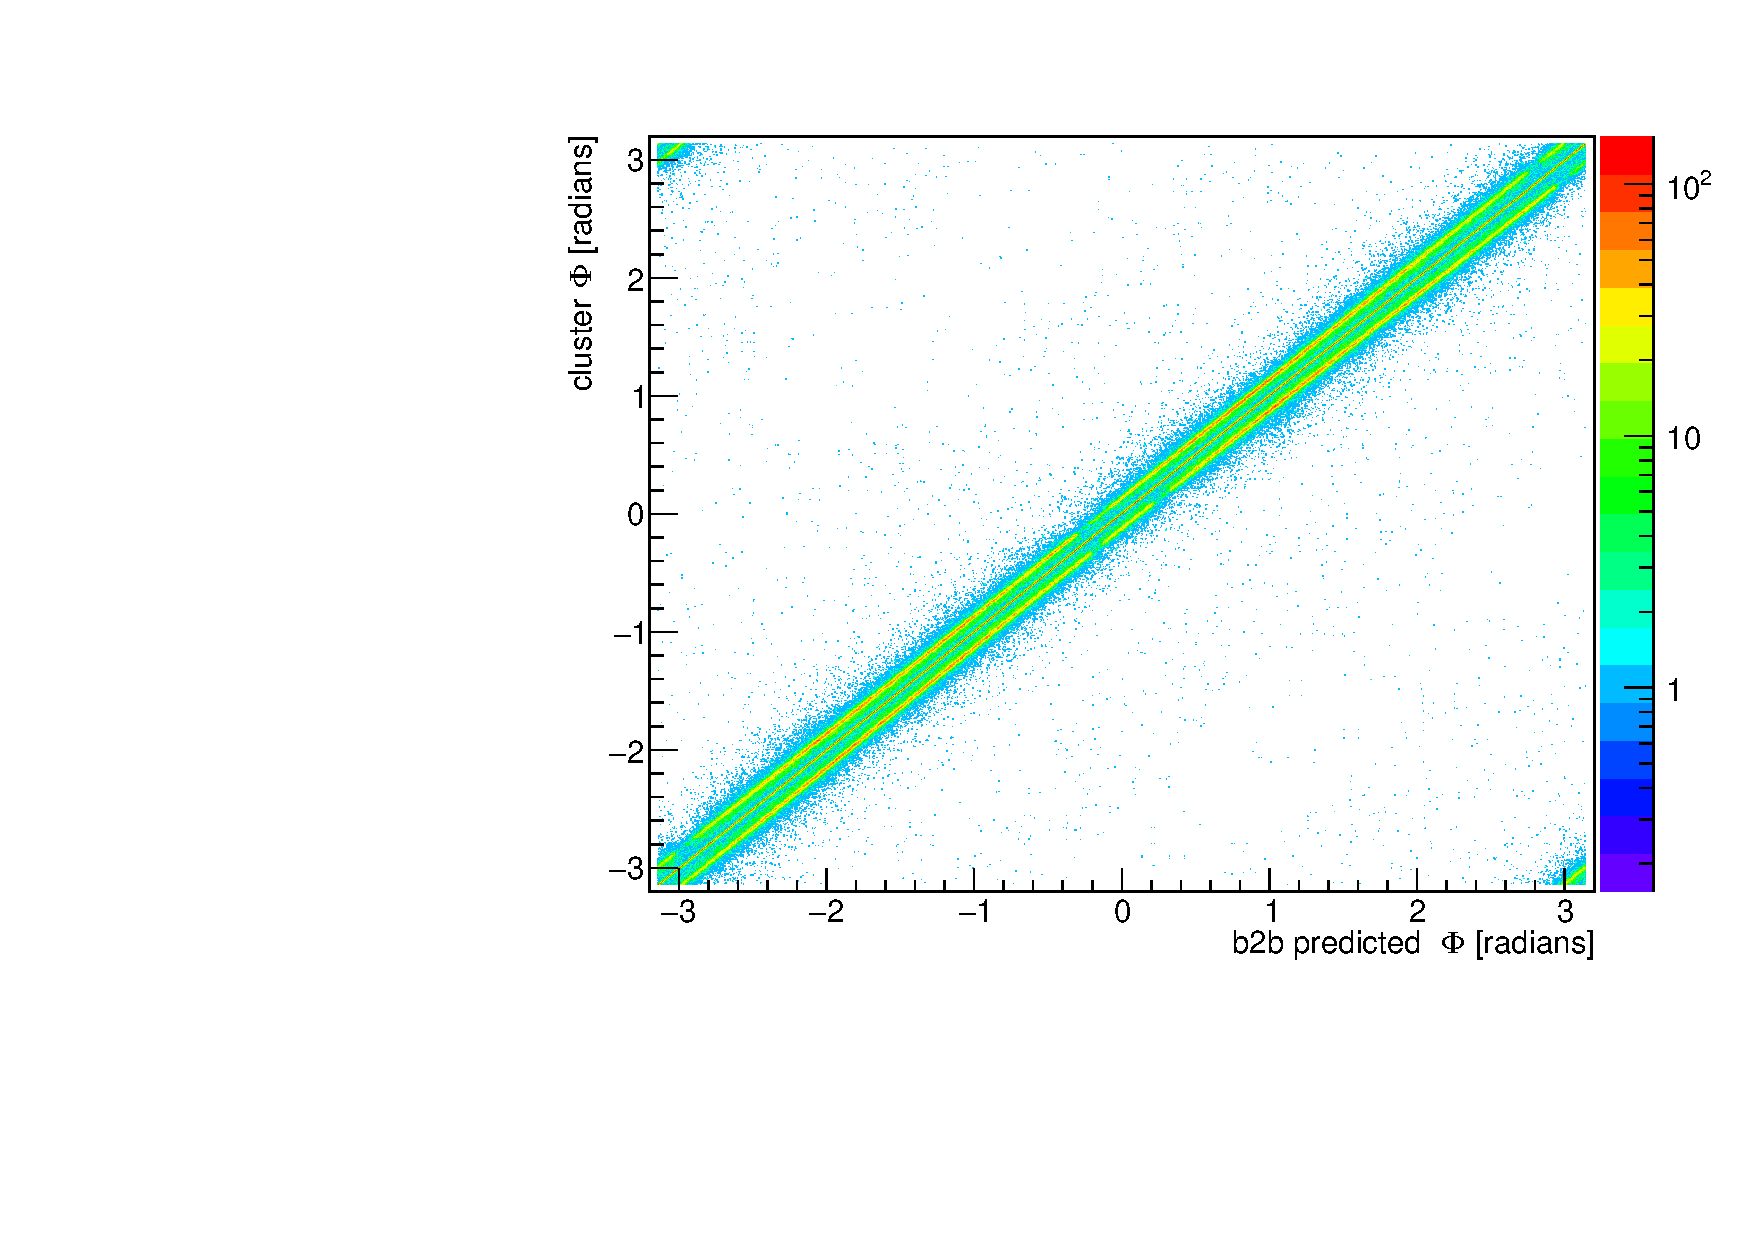
\includegraphics[width=5cm]{Plots/clusterb2b}
			
			\label{fig:sub2}
		\end{subfigure}
				
		\label{fig:test}
	\end{figure}
	
	
\end{frame}


\begin{frame}{Reproducing Plots}
	
	Same plots but zoomed in:
	
		\begin{figure}
		\centering
		\begin{subfigure}{.5\textwidth}
			\centering
			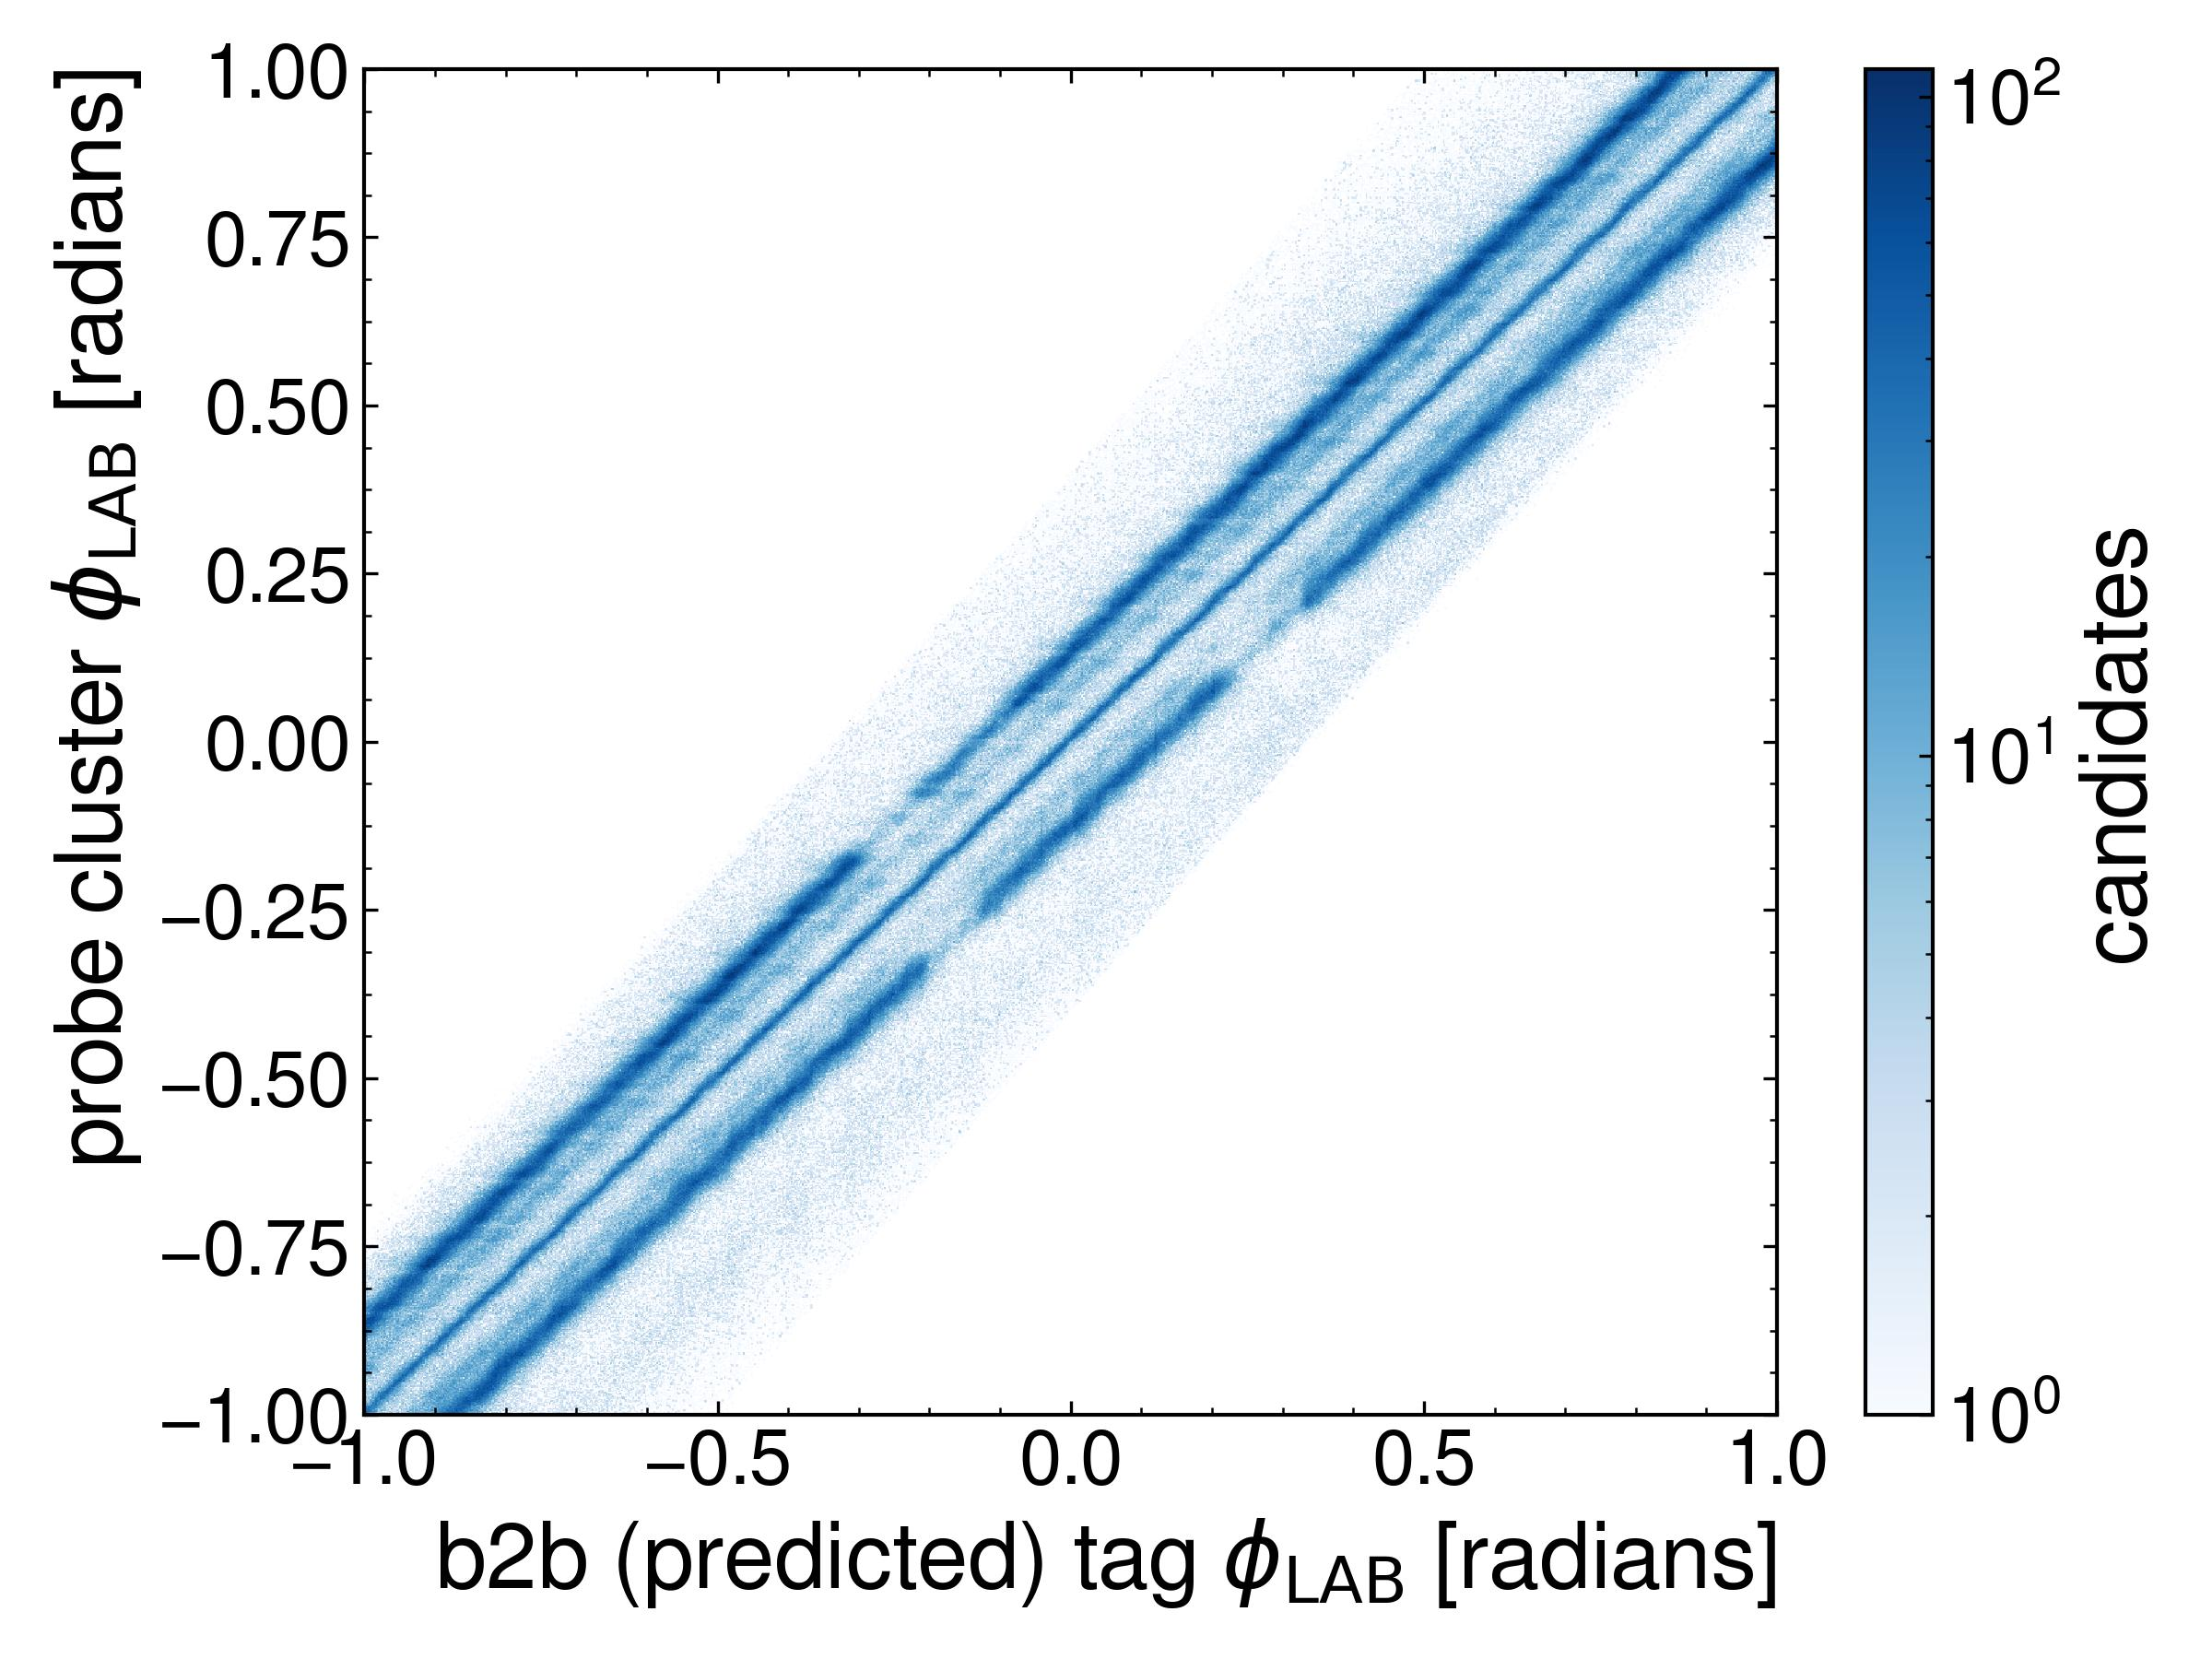
\includegraphics[width=5cm]{Plots/ZommedSam.jpeg}
			
			\label{fig:sub1}
		\end{subfigure}%
		\begin{subfigure}{.5\textwidth}
			\centering
			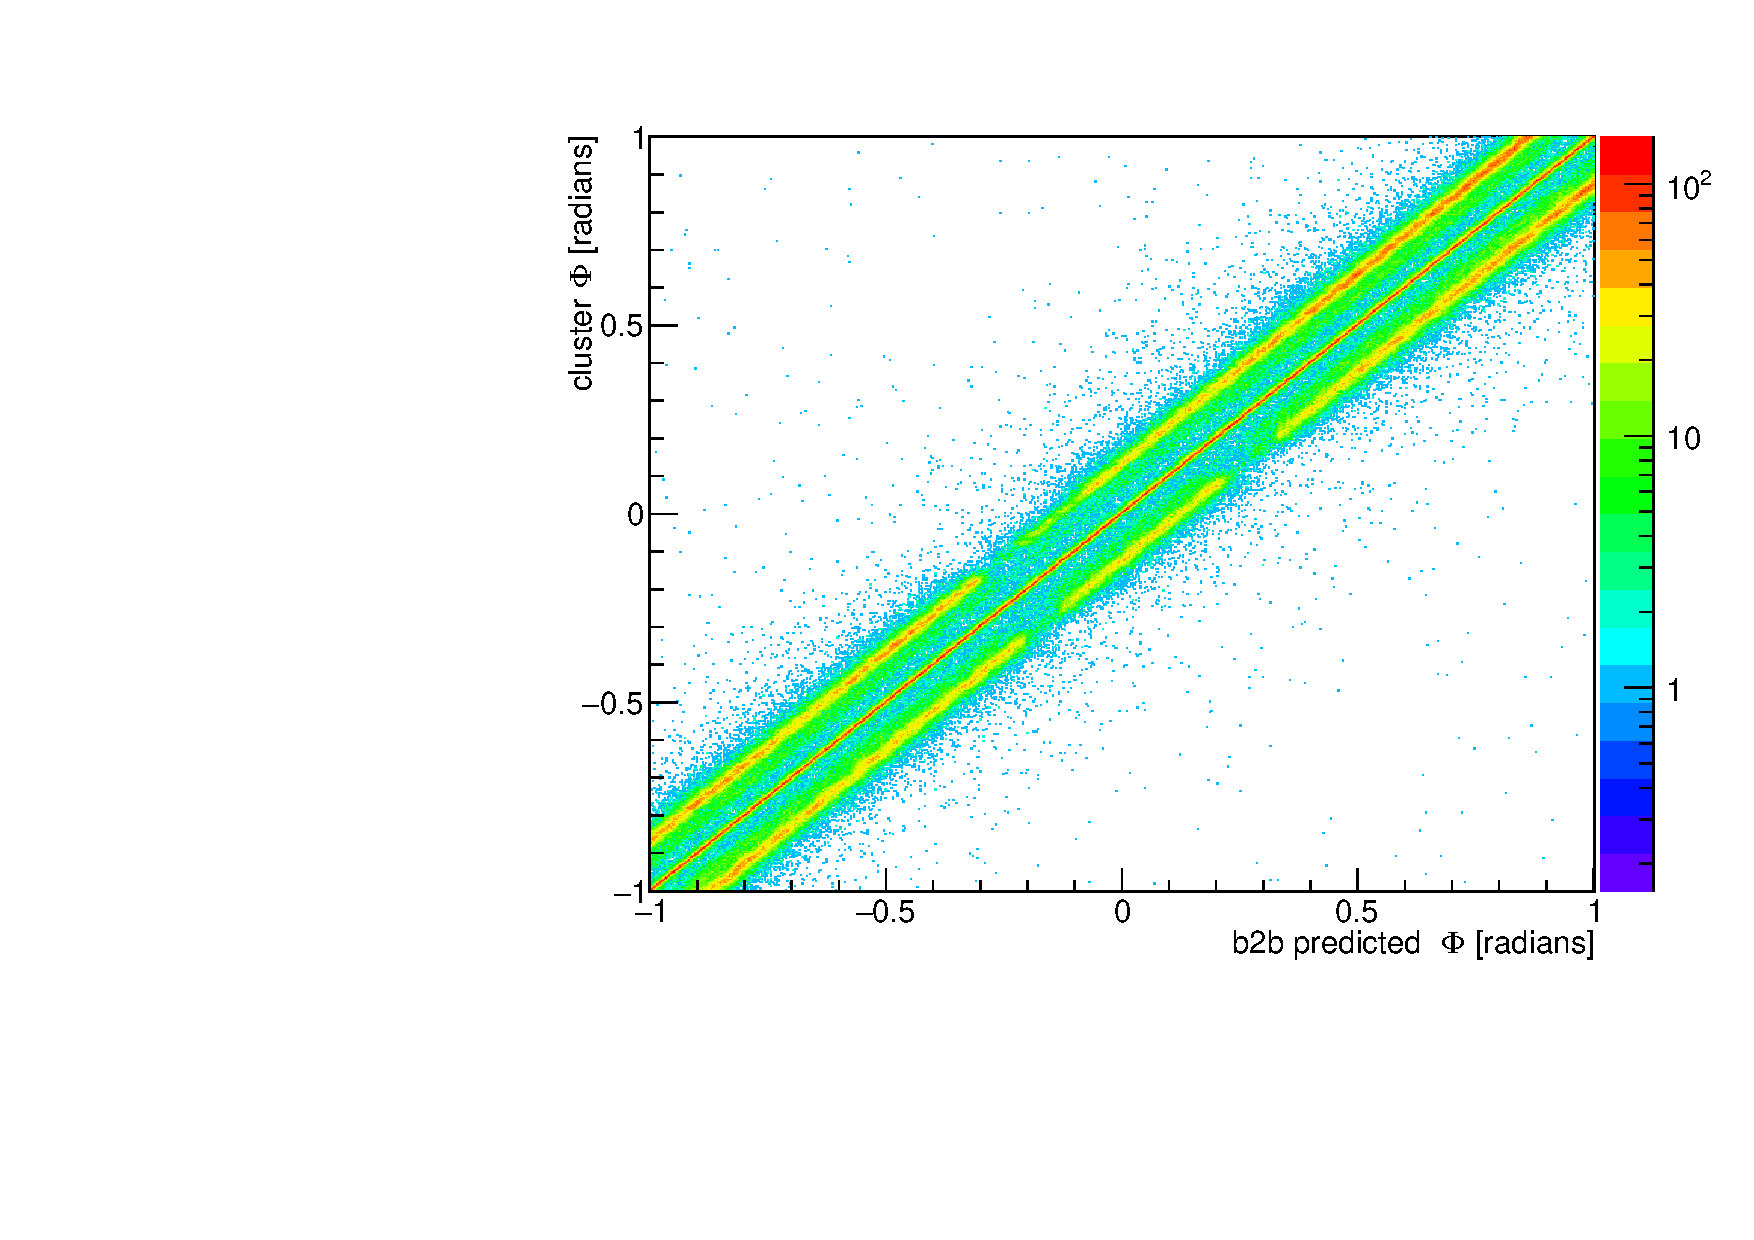
\includegraphics[width=5cm]{Plots/zommedb2b}
			
			\label{fig:sub2}
		\end{subfigure}
		
		\label{fig:test}
	\end{figure}
		
\end{frame}


\begin{frame}{Reproducing Plots}
\begin{itemize} 
	\item The middle peak is $\textrm{ee} \rightarrow \gamma \gamma$, the two other peaks are $\textrm{ee} \rightarrow \textrm{ee}$
	\item My $\textrm{ee} \rightarrow \gamma \gamma$ peak is way higher (Maybe there are some cuts that I am not considering?)

\end{itemize}
\begin{figure}
	\centering
	\begin{subfigure}{.5\textwidth}
		\centering
		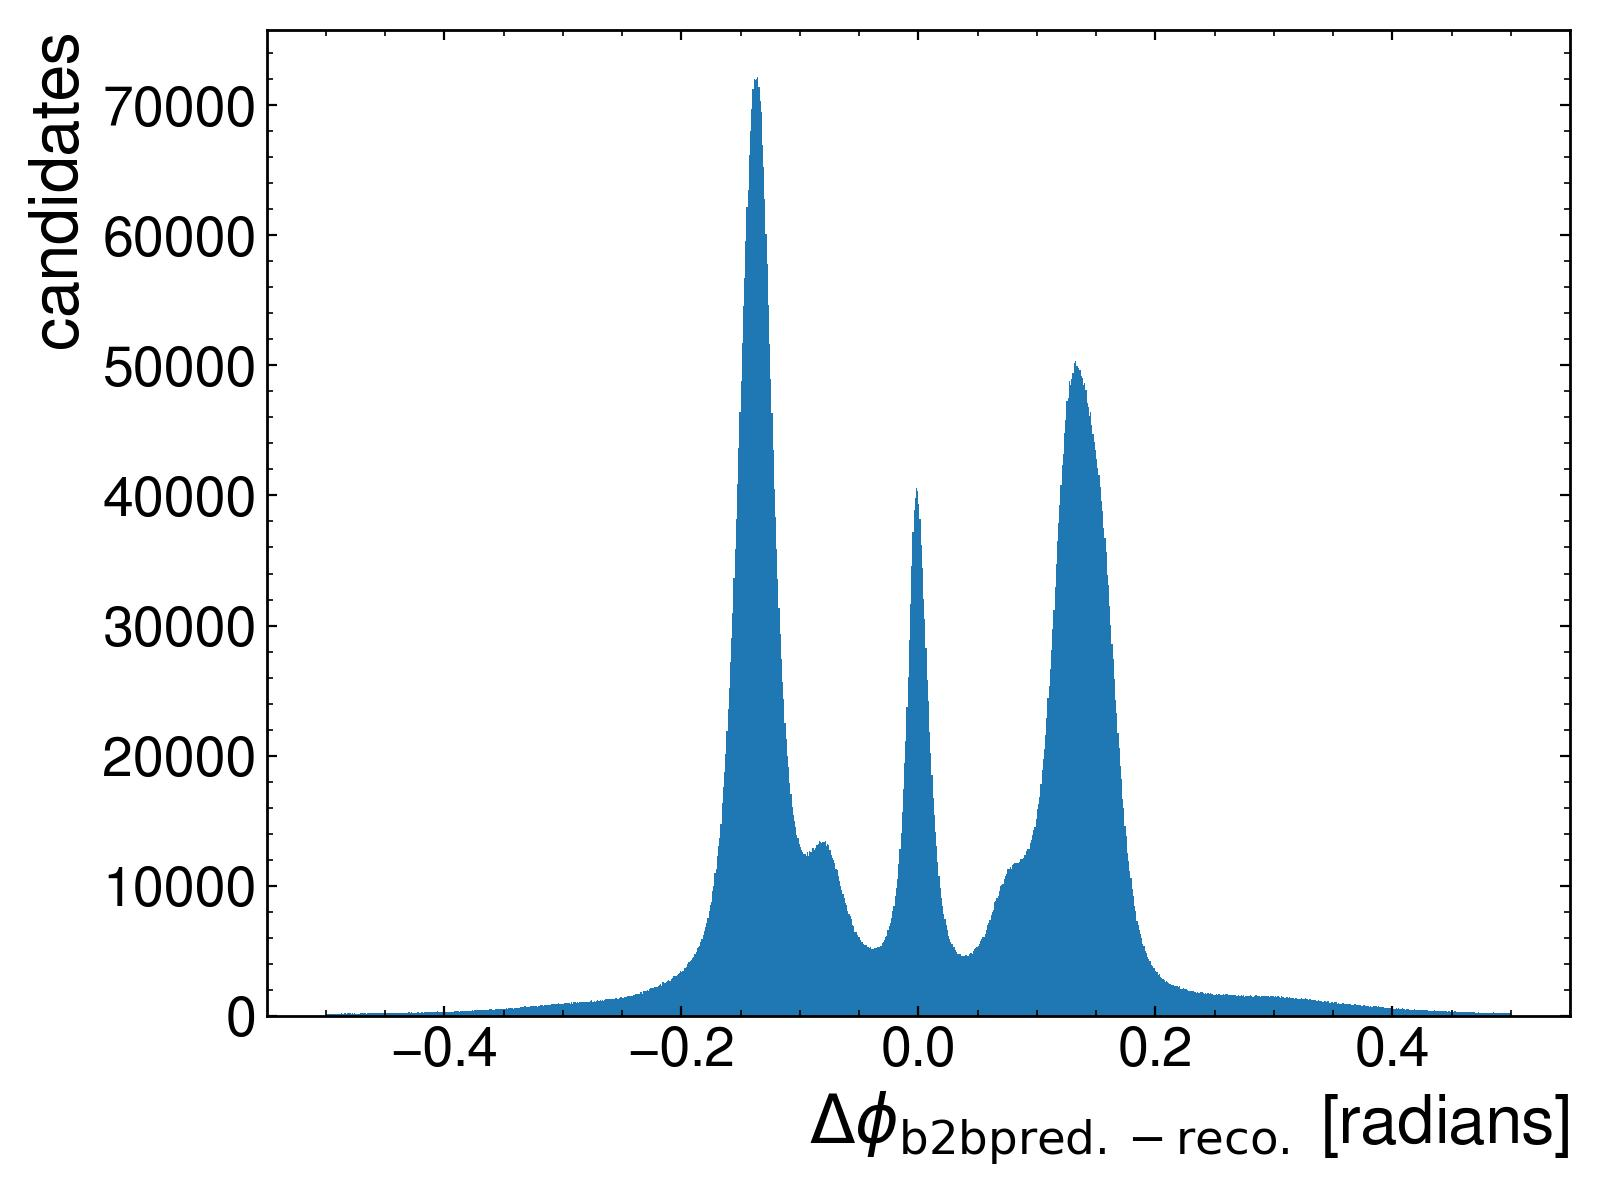
\includegraphics[width=5cm]{Plots/deltaPhiSam.jpeg}
	
		\label{fig:sub1}
	\end{subfigure}%
	\begin{subfigure}{.5\textwidth}
		\centering
		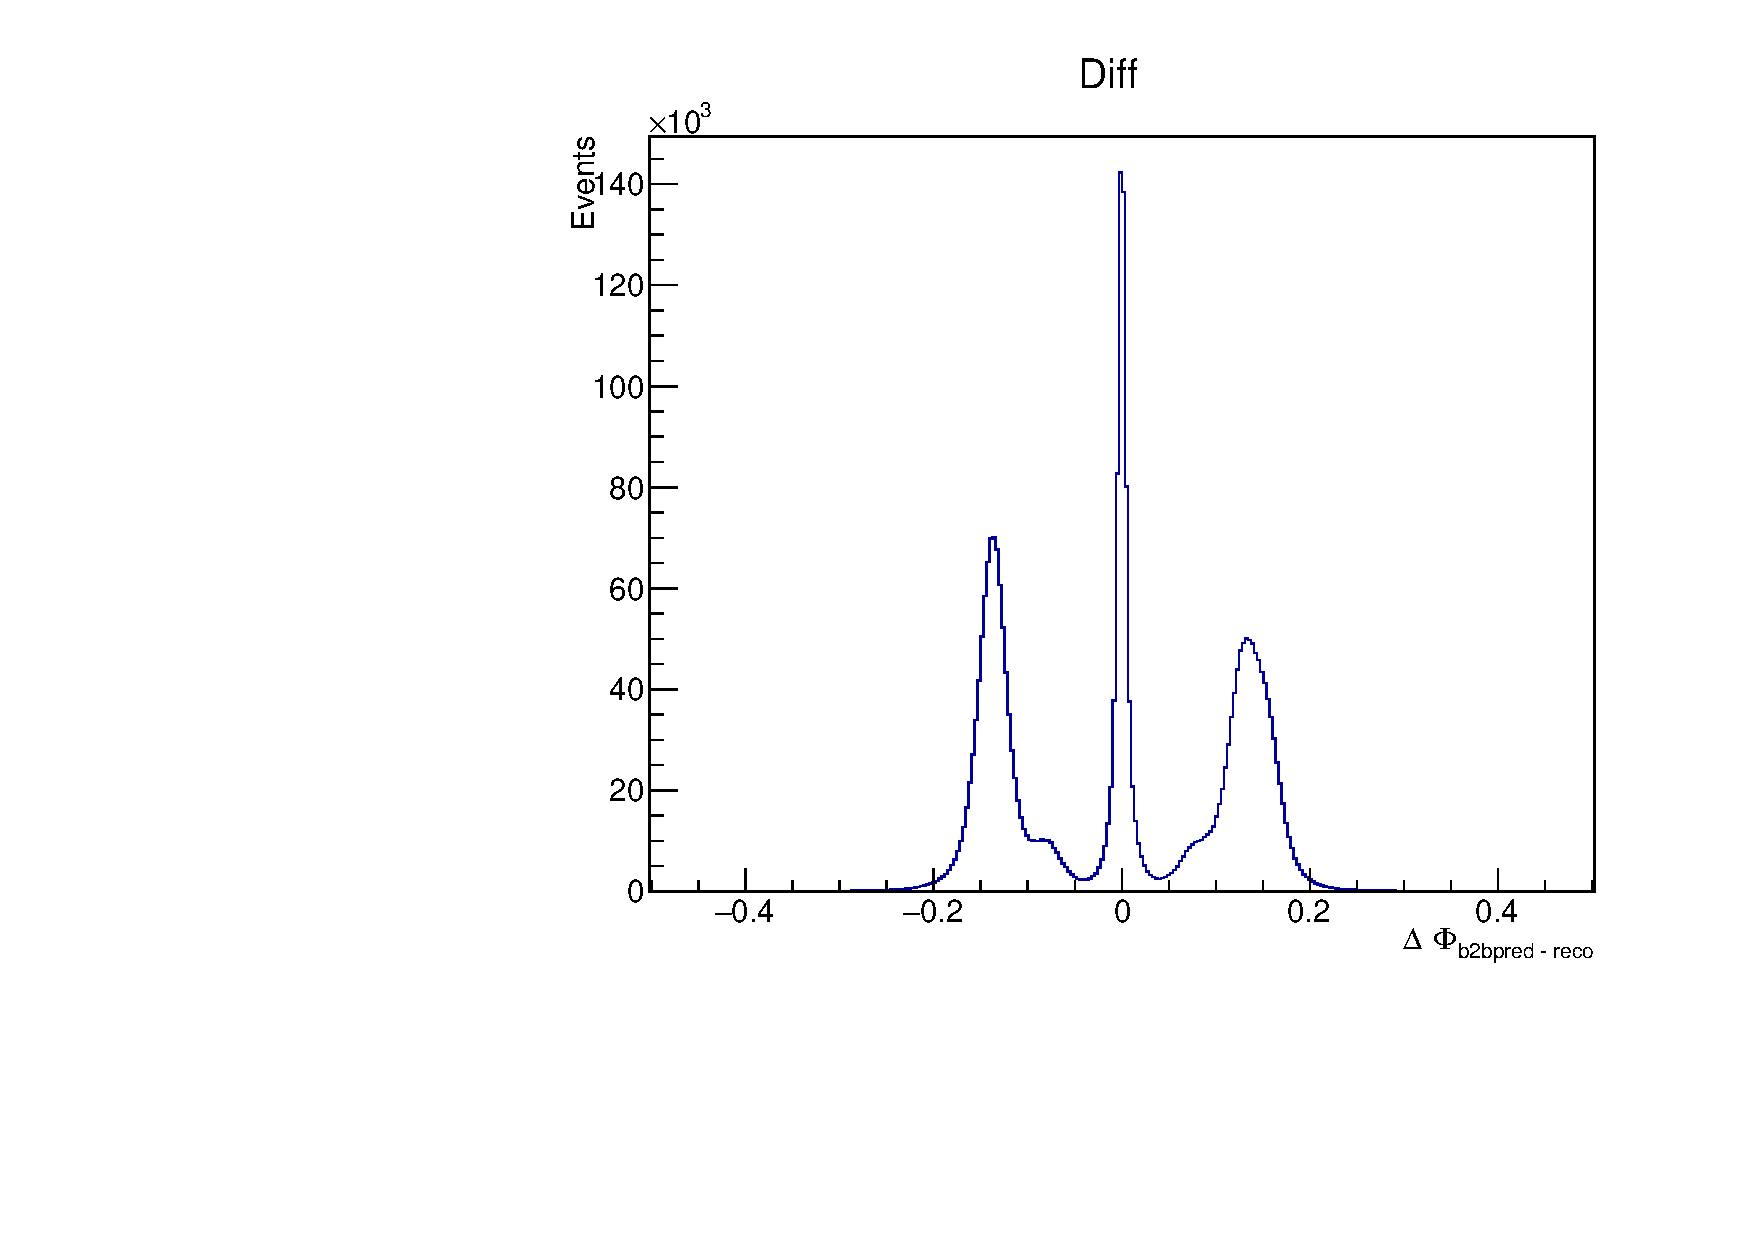
\includegraphics[width=5cm]{Plots/DeltaPhi.pdf}
	
		\label{fig:sub2}
	\end{subfigure}

	\label{fig:test}
\end{figure}

\end{frame}


\begin{frame}{Some more plots}

Here the invariant mass of the virtual photon (vpho) is plotted 

	
	\begin{figure}
		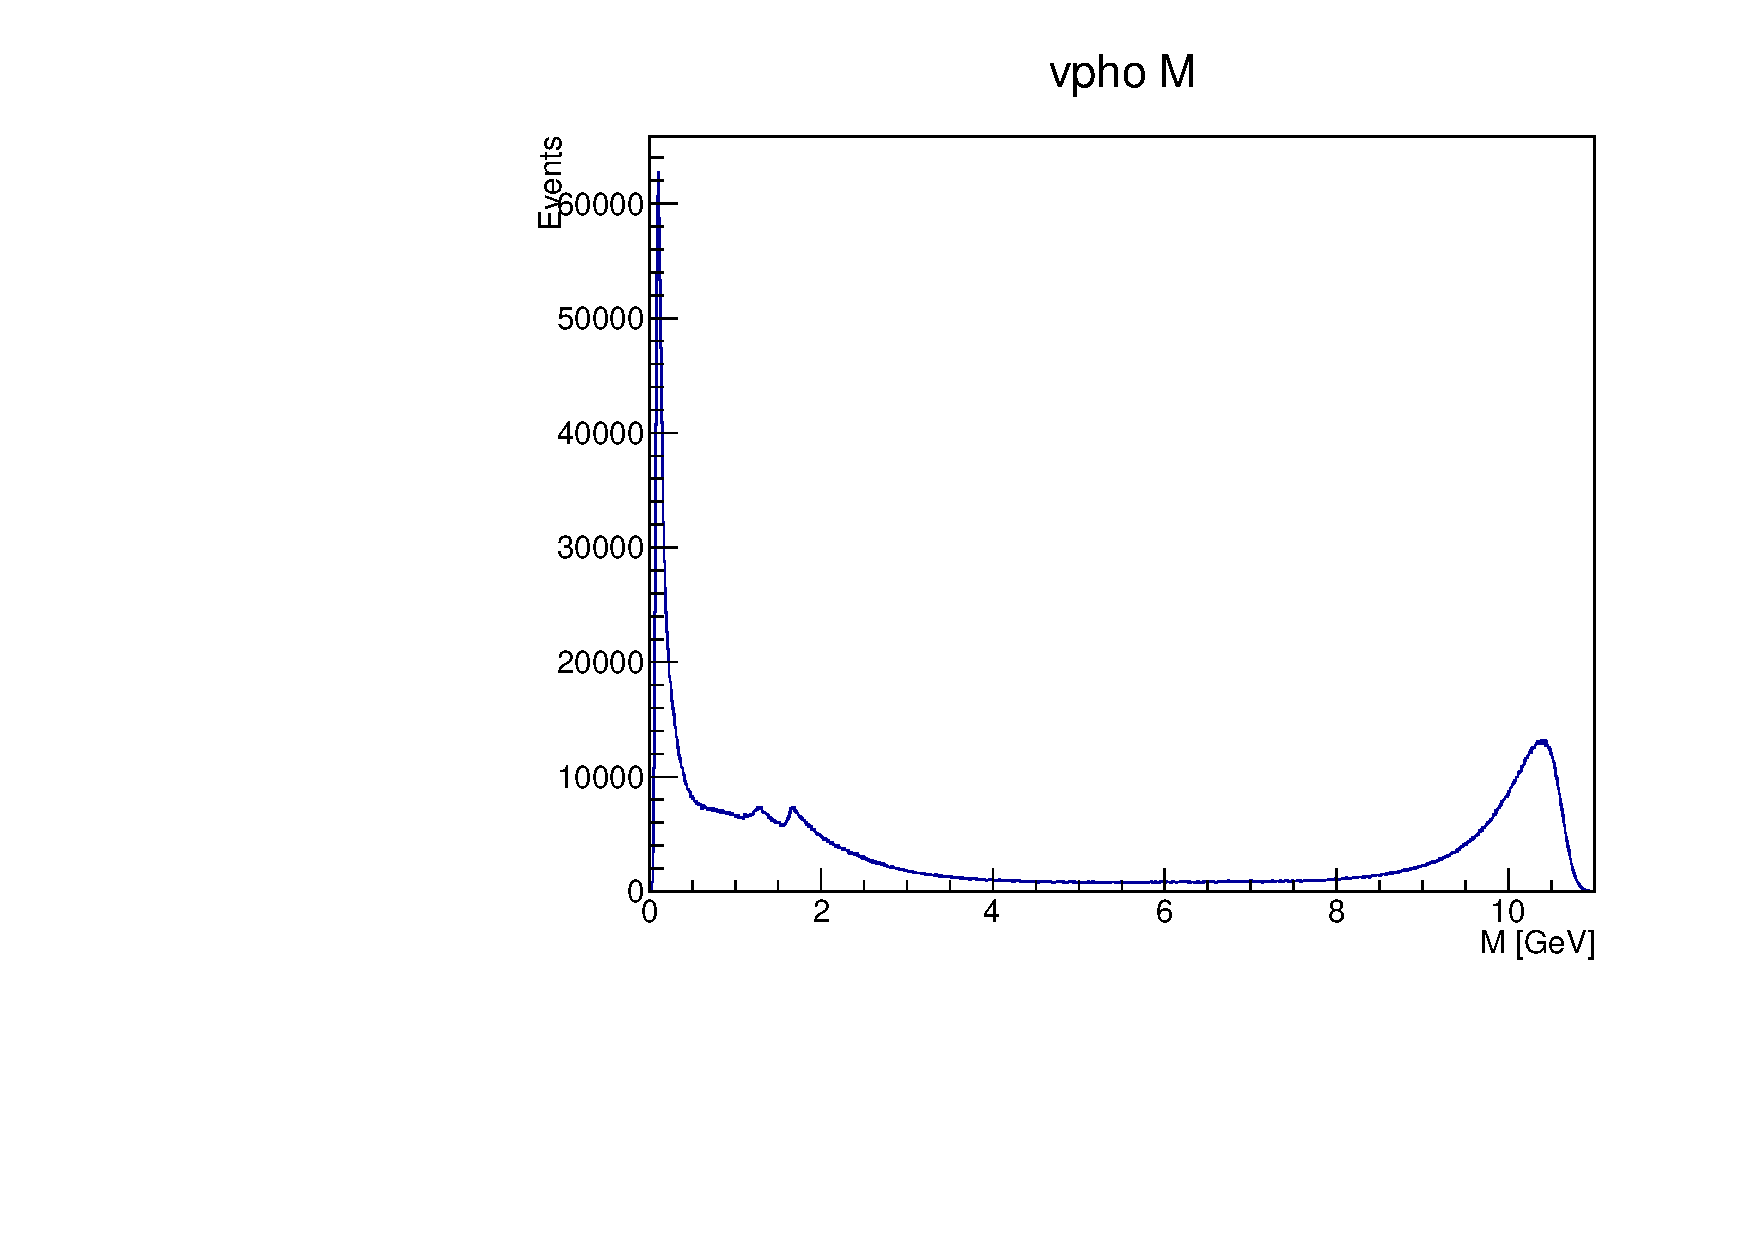
\includegraphics[width=8cm]{Plots/vphoM.pdf}
	\end{figure}
	
	
\end{frame}



\begin{frame}{Some more plots}

	Here the invariant mass of the virtual photon is plotted against the difference between the b2bpredicted and the reconstructed $\Phi $ angel
	\begin{figure}
		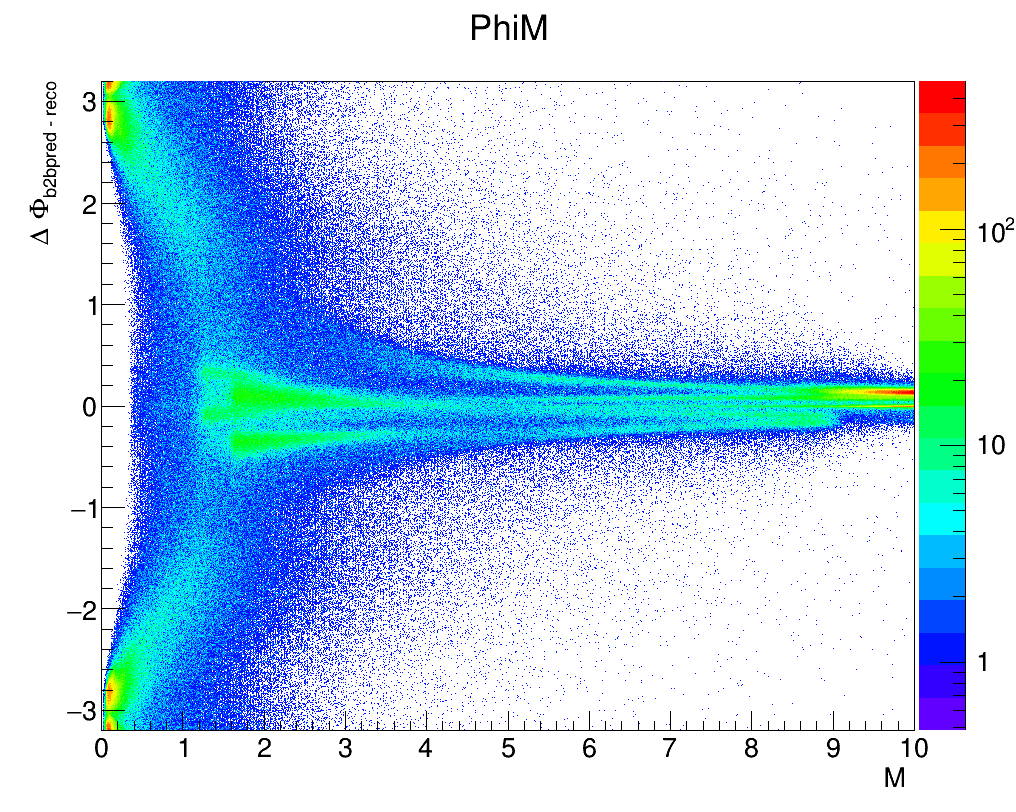
\includegraphics[width=8cm]{Plots/PhiM.png}
	\end{figure}
	
	
\end{frame}

\begin{frame}{Some more plots}
	Here the invariant mass of the virtual photon is plotted against the number of reconstructed Tracks.
	\begin{figure}
		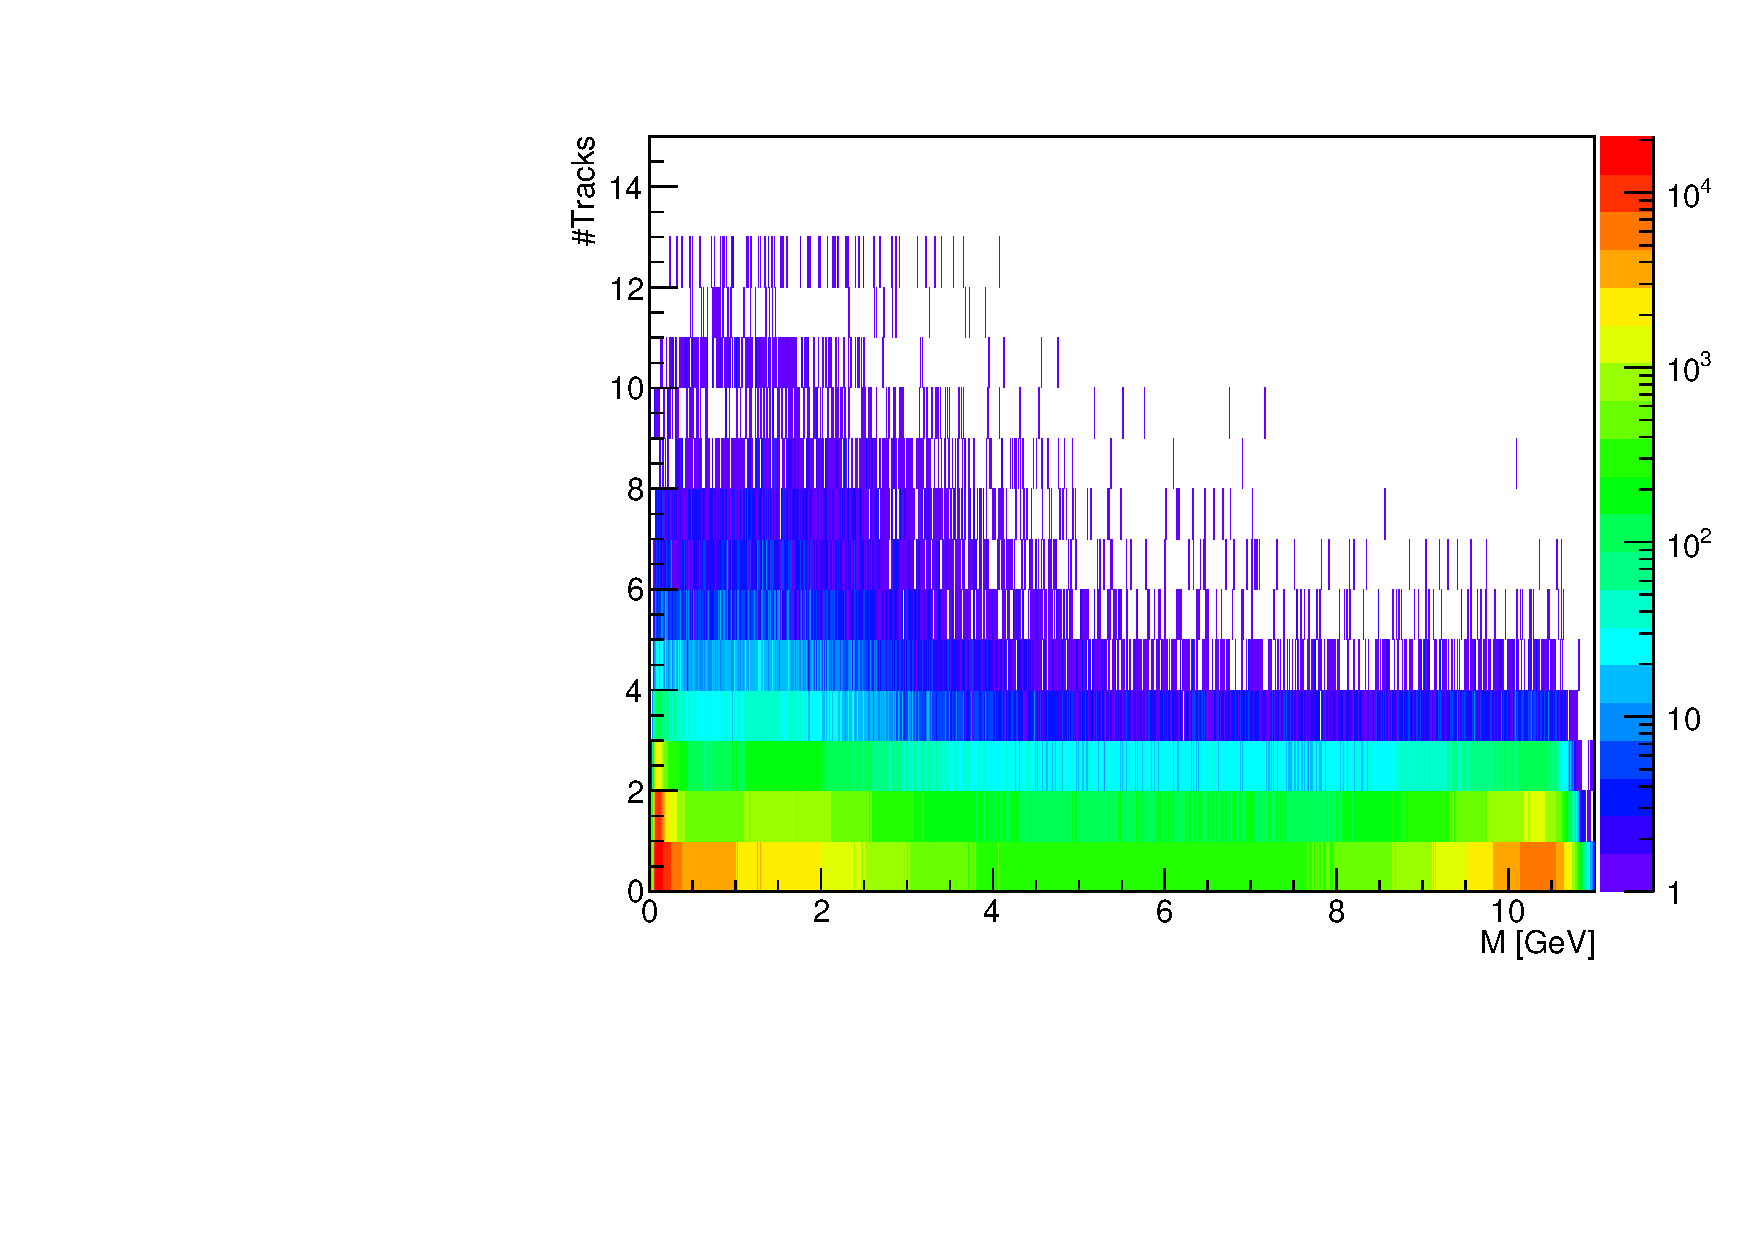
\includegraphics[width=8cm]{Plots/nTrM}
	\end{figure}
	
\end{frame}

\begin{frame}{The next Steps}
	\begin{itemize}
		\item Investigate the best cuts for our purposes and apply them
		\item Select only the $\textrm{ee} \rightarrow \textrm{ee}$ candidates and study the tracking efficiency using that sample
		\item Produce the same plots shown here using MC sample (from a preliminary study using MC10 it looks like very few events survive applying the described selection)
	\end{itemize}
\end{frame}


\end{document}
